\section{Introduction}
\label{sec:introduction}

\subsection{Hall Effect}
\label{sec:intr:hall}
The Hall effect refers to an effect when an electrical conductor lies within a magnetic field. 

The underlying effect is the Lorentz force
\[
  \mathbf F = q (\mathbf E + \mathbf v \times \mathbf B)
\]
which acts as a force on a charge moving through a magnetic field. The force itself is perpendicular
to both the direction of movement and the magnetic field. The later observation also holds for the
voltage measurable with the Hall effect.

One can derive the voltage to be 
\begin{equation}
  U_\text{H} = R_\text{H} \frac{I B}{d}.
\end{equation}
A possible setup for the experiment is shown in \autoref{fig:setup}, where the variables are used
similarly. 
\begin{figure}
  \centering
  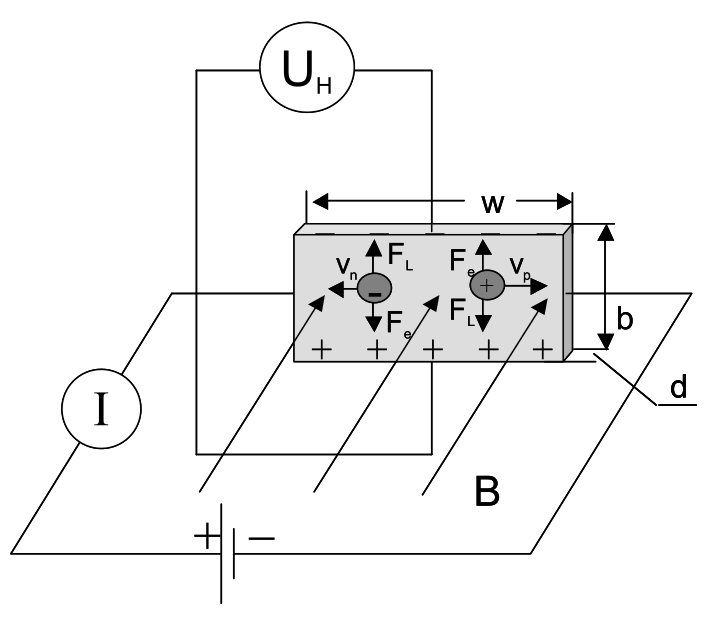
\includegraphics[width=0.4\textwidth]{media/setup_sketch.png}
  \caption{Sketch of an experimental setup to measure the Hall voltage $U_\text{H}$.}
  \label{fig:setup}
\end{figure}

